% Set title page for separate titlepage
\documentclass[titlepage]{report}

%---------% Packages %---------%
% Some standard math packages
\usepackage{amsmath}
\usepackage{amssymb}
\usepackage{amsfonts}
\usepackage{amsthm}
\usepackage{IEEEtrantools}

% Package for lists
\usepackage[shortlabels]{enumitem}

% Graphics
\usepackage{tikz}
\usetikzlibrary{fit,
						backgrounds,
						arrows,
						decorations.markings,
						decorations.pathmorphing,
						snakes,
						shapes.misc, 
						positioning,
						scopes}

\tikzset{colorbox/.style={thick, rounded corners=2pt, text height=1.7ex,text depth=.25ex, draw=#1!70!black, fill=#1!30}}

\tikzset{colorelement/.style={thick, rounded corners=2pt, draw=#1!70!black, fill=#1!30}}
\tikzset{conn/.style={thick, shorten <=#1, shorten >=#1}}
\tikzset{arr_node/.style={pos=0.5,above,font=\scriptsize, sloped}}

\usepackage{float}

% Utilities
\usepackage{lipsum}
\usepackage{arydshln}

% Biblatex
\usepackage[backend=biber,style=numeric,sorting=none]{biblatex}
\nocite{*}
\addbibresource{bib/references.bib}
%------------------------------------%

% Math environments
\theoremstyle{remark}
\newtheorem{remark}{Remark}
\newtheorem{xmpl}{Example}

%quantum commands
\renewcommand{\H}{\mathcal{H}}
\newcommand{\ket}[1]{|#1 \rangle}
\newcommand{\bra}[1]{\langle #1|}
\newcommand{\braket}[2]{\langle#1|#2\rangle}
\newcommand{\bk}[2]{\langle#1|#2\rangle}
\newcommand{\ketbra}[2]{|#1 \rangle\langle #2|}
\newcommand{\kb}[2]{|#1 \rangle\langle #2|}
\newcommand{\proj}[1]{|#1\rangle\langle #1|}

%Math commands
\DeclareMathOperator{\Tr}{Tr} % Trace
\DeclareMathOperator{\Ent}{H} % Entropy
\DeclareMathOperator{\I}{I} % Mutual Information

%------------------------------------%

%\title{
%	{\Huge{\textbf{Bound Entanglement and Bound Information}}}\\
%	{\large{Universit\`a della Svizzera Italiana}}\\
%	{\normalsize{Department of Informatics}}\\
%	\bigskip\medskip
%	{
\includegraphics[scale=0.12]{images/usi-immagini-logo-formatted.png}}
%}
%
%\author{\textbf{Luca Dolfi} \\ \\ Advisor: Prof. Dr. Stefan Wolf \\ \\ Tutor: MSc Arne Hansen}
%\date{Spring 2018}

\begin{document}
%\maketitle
\begin{titlepage}
    \begin{center}
        \vspace*{1cm}
        
        \Huge
        \textbf{Bound Entanglement and Bound Information}
        
        \vspace{0.5cm}
        \LARGE
        Thesis Subtitle
        
        \vspace{1.5cm}
        
        \textbf{Luca Dolfi}\\ 
         Advisor: Prof. Dr. Stefan Wolf \\ 
         Tutor: MSc Arne Hansen \\
        
        \vfill
        
        A thesis presented for the degree of\\
        BSc in Informatics
        
        \vspace{0.8cm}
        
        
\includegraphics[width=0.2\textwidth]{images/usi-immagini-logo-formatted.png}
        
        \Large
        Department of Informatics\\
        Universit\`a della Svizzera Italiana\\
        Spring 2018
        
    \end{center}
\end{titlepage}
%\chapter*{Abstract}
%\lipsum[1]
%\chapter*{Acknowledgements}
%\lipsum[13]
\tableofcontents

%\chapter{Introduction}
%
%\lipsum[1]

	\begin{figure}[H]
		\centering
		% Image of the big idea of the thesis
% discussed also for initial presentation
% should show the "track" that goes from
% QM(bound entanglement) to Classical bound information
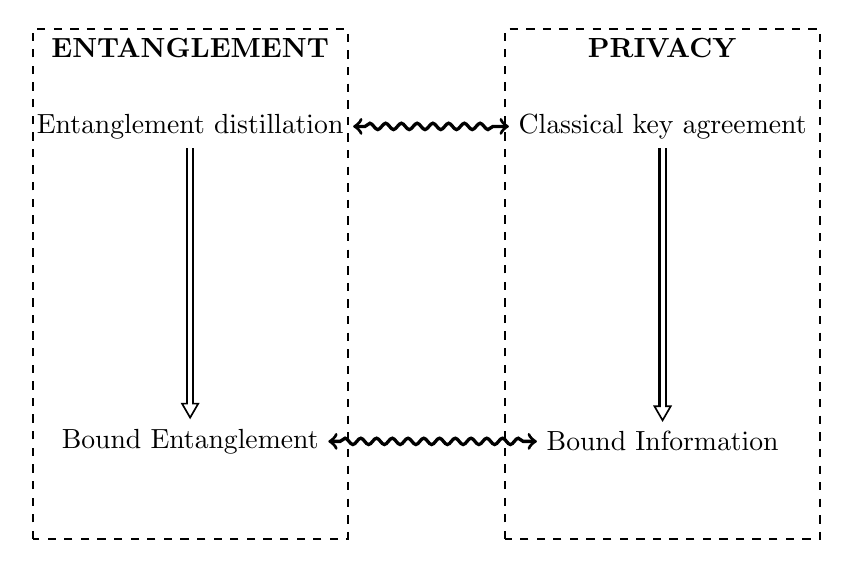
\begin{tikzpicture}
\tikzstyle{vecArrow} = [thick, decoration={markings,mark=at position
   1 with {\arrow[semithick]{open triangle 60}}},
   double distance=1.4pt, shorten >= 5.5pt,
   preaction = {decorate},
   postaction = {draw,line width=1.4pt, white,shorten >= 4.5pt}]
\tikzstyle{fancyArrow} = [<->,very thick,decorate,decoration={snake,amplitude=.4mm,segment length=2mm,post length=1.5mm, pre length=1.5mm}]

  \draw[thick,dashed] (-5,-3.24) rectangle (-1, 3.24);
  \draw[thick, dashed] (1,-3.24) rectangle (5, 3.24);

  \node[below right, anchor=center] (en) at (-3, 3)  {\textbf{ENTANGLEMENT}};
  \node[below right, anchor=center] (pr) at (3, 3)  {\textbf{PRIVACY}};
  \node[below right, anchor=center] (dist) at (-3, 2)  {Entanglement distillation};
  \node[below right, anchor=center] (cka) at (3, 2)  {Classical key agreement};
  \node[below right, anchor=center] (be) at (-3, -2)  {Bound Entanglement};
  \node[below right, anchor=center] (bi) at (3, -2)  {Bound Information};
  \draw[vecArrow] (dist) to (be);
  \draw[vecArrow] (cka) to (bi);
  \draw[fancyArrow] (dist) to (cka);
  \draw[fancyArrow] (be) to (bi);

\end{tikzpicture}

		\caption{the big picture that represents how QM and Information Theory can relate to each other}
	\end{figure}
	\begin{table}[ht]
	 \centering
	 	\begin{tabular}{ l | l}
	 		\textbf{entanglement theory} & \textbf{key agreement} \\ 
	 		\hline 
	 		quantum entanglement & secret classical correlations \\ 
	 		quantum communication & secret classical communication \\ 
	 		classical communication & public classical communication \\ 
	 		local actions & local actions \\ 
	 	\end{tabular} 
	 	\caption{Table taken from \cite{4H07}}
	 \end{table}
	
	
	\section{Motivation}
	Why doing it. \\
	from where does the intuition come from $\rightarrow$ explain intuition\\
	why it may be useful\\
	Looking at QM $\rightarrow$ WHY\\
	Utilities in real world.\\
	
	%maybe a bit of an overstatement, but we are dealing the most secure privacy possible, right?
	\begin{quote}
	\textbf{Computational security (RSA)$<$ security through physical laws (BB84)$<$ information theoretical security (??)}
	\end{quote}
	
	\begin{quotation}
	It is interesting, that entaglement, which is originally quantum concept, corresponds to privacy in general - not only in the context of quantum protocols.
	\footcite{4H07}
	\end{quotation}
	\begin{quotation}
	The task of Alice and Bob is to obtain via local (classical) operations and public communication (LOPC) the longest bit-string which is almost perfectly correlated and about which Eve (who can listen to the public discussion) knows a negligible amount of information.
	\footcite{4H07}
	\end{quotation}		
	
	\begin{figure}[H]
		\centering
		% Image showing intuition process
% Sort of justify how and why 
% bound entanglement and bound information
% should share analogies

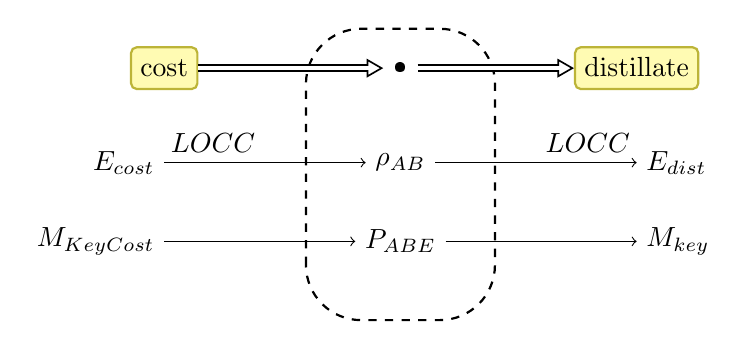
\begin{tikzpicture}
\tikzstyle{vecArrow} = [thick, decoration={markings,mark=at position
   1 with {\arrow[semithick]{open triangle 60}}},
   double distance=1.4pt, shorten >= 5.5pt,
   preaction = {decorate},
   postaction = {draw,line width=1.4pt, white,shorten >= 4.5pt}]
\tikzstyle{fancyArrow} = [<->,very thick,decorate,decoration={snake,amplitude=.4mm,segment length=2mm,post length=1mm}]

	\coordinate (center) at (0,0);
	\draw[thick,dashed,rounded corners=.7cm] (-1.20,-1.5) rectangle (1.20, 2.2);
	\node[colorbox=yellow] (cst) at (-3,1.7) {\strut cost};
	\node[colorbox=yellow, baseline=(cst.baseline)] (dst) at (3,1.7) {\strut distillate};
	\node[anchor=center, left] (ecost) at (-3,0.5) {$E_{cost}$};
	\node[anchor=center] (rho) at (0.0,0.5) {$\rho_{AB}$};
	\node[anchor=center, right] (edist) at (3,0.5) {$E_{dist}$};
	\node[anchor=center, left] (kcost) at (-3,-0.5) {$M_{KeyCost}$};
	\node[anchor=center] (prob) at (0.0,-0.5) {$P_{ABE}$};
	\node[anchor=center, right] (ckey) at (3,-0.5) {$M_{key}$};
	\node[thick, baseline=(cst.baseline)] (bul) at (0.0, 1.7) {\strut\textbullet};
%	\node[above=of bul] (res) {Resource (fixed)}; 
	

	\draw[vecArrow] (cst.east) to (bul.west);
	\draw[vecArrow] (bul.east) to (dst.west);
	\draw[->] (ecost) to node[above left]{$LOCC$} (rho); \draw[->] (rho) to node[above right]{$LOCC$} (edist);
	\draw[->] (kcost) to (prob); \draw[->] (prob) to (ckey);

\end{tikzpicture}

		\caption{Sort of how and why the intuition is constructed from previous knowledge of concepts of QM}
	\end{figure}
	
	\begin{quotation}
	[...] an analogue of the necessary and sufficient condition for entanglement distillation was found.
	As in the quantum case the state is distillable iff there exists a projection (acting on $n$ copies of a state for some $n$) onto 2-qubit subspace which is entangled, 
	in the classical case, the key is distillable iff there exists a binary channel (acting on $n$ copies of a distribution for some $n$) which outputs Alice's and Bob's variables, such that the resulting distribution has nonzero key.
	\cite{4H07}
	\end{quotation}
	
	
	\section{Linear Algebra and Notation}
	
	\begin{enumerate}
	\item Dirac's braket notation
	\item Inner/Outer product
	\item Linear operator
	\item Adjoints and Hermitian operators
	\item Pauli matrices
	\item Tensor Product and tensor space
	\end{enumerate}
	
	\subsubsection*{Inner/outer product}
	The inner product of two vectors $\ket{v}$ and $\ket{w}$ is
	$$ ( \ket{v} , \ket{w} ) = \bk{v}{w} = (\ket{w} , \ket{v} )^{\ast} = \bk{w}{v}^{\ast} $$
	Where $\ast$ represents the transpose, and because we are dealing with complex number, we also intend the conjugate transpose,	which produces a scalar (complex) value.\\ %real??
	This property is foundamental in the sense that it will allows us to go from a state space --that can be many dimensional-- to a \textit{measurement} space, which assumes real values.\\ %0 and 1 in our case??
	In standard vector notation this is no different from
	$$ ( \vec{v}, \vec{w} ) =  \begin{pmatrix} \bar{v_1} & \bar{v_2}\end{pmatrix} \begin{pmatrix} w_1 \\ w_2 \end{pmatrix} = \begin{pmatrix} \bar{w_1} & \bar{w_2}\end{pmatrix} \begin{pmatrix} v_1 \\ v_2 \end{pmatrix} = ( \vec{w}, \vec{v} )^{\ast}$$
	It is important also to note that through the inner product of two vectors we also define the norm $\Vert\ket{v}\Vert  =  \sqrt{\braket{v}{v}} $.\\
	
	
	The outer product of two vectors, on the other hand, produces a matrix, with very important properties. So if we define the matrix\footnote{The fact that the result of  $ \ketbra{w}{v} $ is indeed a matrix can be seen more directly if we remember that this is nothing less than a coloumn-row vectors multiplication.} $A =  \ketbra{w}{v} $ we observe that
	$$ \ket{w}\braket{v}{v'} = \braket{v}{v'}\ket{w} $$	
	which is a really convenient way of visualizing the action of matrix $A$. In particular if we divide it like $(\ketbra{w}{v}) (\ket{v'}) $ it is easy to interpret it as \textit{matrix $A$ acting on vector $\ket{v'}$}; but the other equivalent form $(\braket{v}{v'})(\ket{w})$ can also be seen as multiplying vector $\ket{w}$ by a value $\braket{v}{v'}$. \\
	%this part may be too similar to book, page 67...
	The meaning of this is that $\ketbra{w}{v}$ can indeed be defined as a (linear) operator from the vector space of $\ket{v}$ and $\ket{v'}$ to the vector space of $\ket{w}$. This comes in very handy when we later use it to define operations and measurements on quantum states. % is this true?
	
	\subsubsection*{Linear operators}
	A linear operator between two vector spaces is defined as 
	$$ \mathbf{A}: V\longrightarrow W \text{  ,  }\ket{v_i}\mapsto A\ket{v_i}$$
	$$ \text{ linear in all inputs, i.e.  }  A\left( \sum_i a_i\ket{v_i}\right) = \sum_i a_i A\ket{v_i} \text{  for all } i $$ 
	Looking back at the definition of the matrix $ A = \ketbra{w}{v}$ we can now refer to it as a linear operator from now on.
	
	\section{Basics of QM}
	\begin{quotation}
		The simplest quantum mechanical system, and the system which we will be most concerned with, is the \emph{qubit}. A qubit has a two-dimensional state space. [...] 
		The way a qubit differs from a bit is that superpositions of these two states, of the form $a\ket{0} + b\ket{1}$, can also exist, in which it is not possible to say that the qubit is definitely in the state $\ket0$, or definitely in the state $\ket1$.
		\cite{QC10th}
	\end{quotation}
	
	%%TODO review this
	All pure states in QM are normalized vectors in $\H$.
	$$ \ket{\psi}\in\H \Rightarrow  \vert\bk{\psi}{\psi}\vert = 1$$
	This is instrumental in seeing them as probability vectors. Every linear operator has then to be unitary to maintain this property.\\
	A statistical mixture of states corresponds to a \emph{density matrix}, which is itself a new state. It is important to note that a mixture of probability of states is not the same thing as superposition of states. In the latter we don't have a measure of uncertainty of the state, meaning also that in theory we are always able to find a measurement basis that will always output the same result for that state. In the former, however, this is not possible given by the direct intrinsic uncertainty of the state.\\
	Density matrices have then the properties:
	$$ M = \rho = \sum_i p_i \ketbra{\psi_i}{\psi_i} = \sum_i p_i P_{\ket{\psi_i}} \text{  , where state }\ket{\psi_i}\text{ has probability } p_i $$ 
	$\rho$ is a positive, trace-1 operator meaning that $Tr(\rho) = 1$ and all eigenvalues of $\rho$ are positive. Moreover $\rho$ is a linear combination of projectors $\ketbra{i}{i}$ which makes $\rho\in\mathbf{P}(\H)$ a projector itself on the the Hilbert space.
	
	
	\begin{figure}[ht]
		\centering
		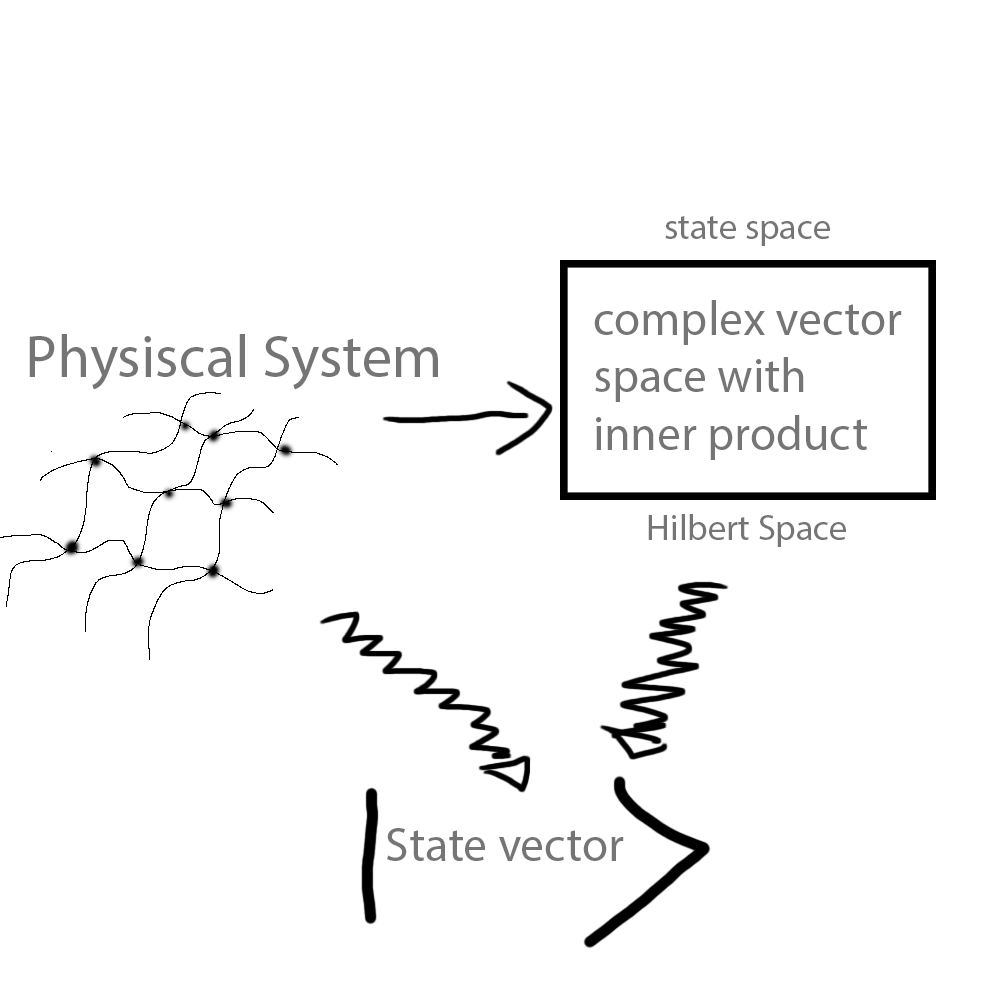
\includegraphics[scale=0.2]{images/sketch1.png} 
		\caption{how a physical state is represented}
	\end{figure}
	

	
		\subsection{Quantum Entanglement}
		%\lipsum[4]
		\begin{figure}
		\centering
		%% Little schematics showing the origin of entanglement
%% from the linear theory of QM and tensor product

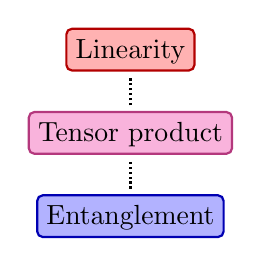
\begin{tikzpicture}[scale=0.6]
  \node[colorbox=red]                      (lin)  {Linearity};
  \node[colorbox=magenta, below=.5cm of lin] (tp)  {Tensor product};
  \node[colorbox=blue, below=.5cm of tp]   (en)  {Entanglement};
  \draw[conn=2pt, densely dotted] (tp) to (lin);
  \draw[conn=2pt, densely dotted] (en) to (tp);
\end{tikzpicture}
		\caption{origin of entanglement via linearity}
		\end{figure}
		
	\section{Basics of Information Theory}
	%\lipsum[3]
		\subsection{Classical Key Agreement}
		%\lipsum[3]

\chapter{Motivation}
% Motivation chapter
% contains also abstract explanation on theoretic secure key distribution

%\lipsum[3]

The goal of key exchange is to allow Alice and Bob to establish a secure, private channel for communication.
For two parties to communicate confidentially, it is first needed to share some secret key between them, so that each party can encrypt and decrypt the communication.
If two parties could not establish a secure --- as in information theoretic secure --- initial key exchange, they cannot communicate with absolute security without the risk of an eavesdropper Eve listening to them.
The ultimate goal of Alice and Bob is to achieve a level of privacy, such that no eavesdropper could have information about the communication, even partially.\\
%The tools or \emph{resources} to obtain such initial common secret can have many shapes and forms in modern telecommunication, often relying on computer science.\\

It has been noticed that these concepts of privacy also appear in nature and the strongest analogy comes from quantum mechanics.\footnotemark 
From this theory arises the famous \emph{quantum entanglement} that appears to be the equivalent of privacy in many ways.
Both phenomena are composed of correlations between known parties that no other person can access or copy. As summed in \cite{4H07} "If systems are in pure entangled state then at the same time (i) systems are correlated and (ii) no other system is correlated with them."
This can be seen as Alice and Bob holding a secret that Eve cannot get to know.
\begin{table}[h]
	 \centering
	 	\begin{tabular}{ l | l}
	 		\textbf{quantum theory} & \textbf{classical information} \\ 
	 		\hline 
	 		(pure) quantum entanglement & secret classical correlations \\ 
	 		quantum communication & secret classical communication \\ 
	 		classical communication & public classical communication \\ 
	 		entanglement distillation & classical key agreement (CKA) \\ 
	 		local actions & local actions \\ 
	 		bound entanglement & bound information ? \\
	 	\end{tabular} 
	 	\caption{Table showing key QM concepts and their analog in classical key agreement, following \cite{CP02}.
	 	\label{Tab:analogy}}
	 \end{table}

\footnotetext{While those analogies are present in many sources, they can be found summed up in the paper by Collins and Popescu \cite{CP02}, which also shortly addresses the question of bound information. }

From table \ref{Tab:analogy} we see that some of the resources and operations of QM have a bijective analog in classical information theory. 
Such a (close) relation suggests that the two theories can be viewed together and to use one to better understand the other. 
It is important however to point out that quantum entanglement and its effects \emph{are not} a quantum manifestation of classical effects and one theory does not prove the other.
There are limitations to the correspondences. 
For example there is no known instance --- and it is believed to not exist -- of a classical correspondence to super-dense coding (a quantum effect). Other entities like a classical correspondence to bound entanglement, \emph{bound information}, are not excluded a priori and remain yet to be observed or disproved.

	\begin{figure}[h!]
		\centering
		% Image of the big idea of the thesis
% discussed also for initial presentation
% should show the "track" that goes from
% QM(bound entanglement) to Classical bound information
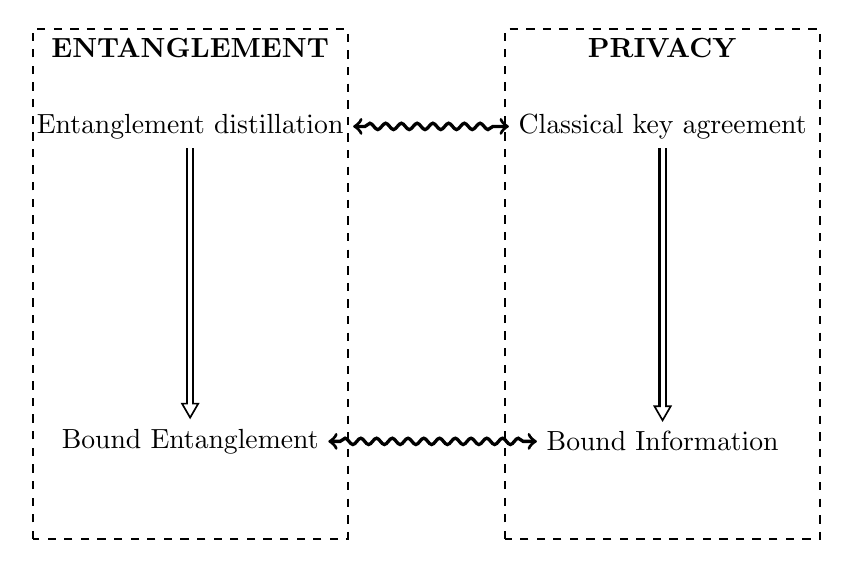
\begin{tikzpicture}
\tikzstyle{vecArrow} = [thick, decoration={markings,mark=at position
   1 with {\arrow[semithick]{open triangle 60}}},
   double distance=1.4pt, shorten >= 5.5pt,
   preaction = {decorate},
   postaction = {draw,line width=1.4pt, white,shorten >= 4.5pt}]
\tikzstyle{fancyArrow} = [<->,very thick,decorate,decoration={snake,amplitude=.4mm,segment length=2mm,post length=1.5mm, pre length=1.5mm}]

  \draw[thick,dashed] (-5,-3.24) rectangle (-1, 3.24);
  \draw[thick, dashed] (1,-3.24) rectangle (5, 3.24);

  \node[below right, anchor=center] (en) at (-3, 3)  {\textbf{ENTANGLEMENT}};
  \node[below right, anchor=center] (pr) at (3, 3)  {\textbf{PRIVACY}};
  \node[below right, anchor=center] (dist) at (-3, 2)  {Entanglement distillation};
  \node[below right, anchor=center] (cka) at (3, 2)  {Classical key agreement};
  \node[below right, anchor=center] (be) at (-3, -2)  {Bound Entanglement};
  \node[below right, anchor=center] (bi) at (3, -2)  {Bound Information};
  \draw[vecArrow] (dist) to (be);
  \draw[vecArrow] (cka) to (bi);
  \draw[fancyArrow] (dist) to (cka);
  \draw[fancyArrow] (be) to (bi);

\end{tikzpicture}

		\caption{Certain aspects of quantum mechanics can be mapped to classical information theory.}
		\label{Fig:bigpicture}
	\end{figure}
An open question has remained over the years asking whether bound information exists in the classical regime.
Should this resource exists, it would be --- by definition --- unusable to generate any key from it.
Nevertheless the existence of a resource with bound information might lead to interesting bounds on information theoretical key exchange.
To summarize, we are interested in the following question:

\paragraph*{The Question}
\begin{itemize}
		\item[] Is there a tripartite probability $P_{ABE}$, corresponding to Alice and Bob wanting to establish a key unknown to Eve, that has some \emph{cost} associated to it to create it, but has $0$ possible key bits extractable from it? 
\end{itemize}


	
		
% Comment out empty chapters
\chapter{Fundamentals}
\section{What is a shared key?}
	The first step towards understanding \emph{bound information} is looking at the end product of a key exchange. 
	The secret key is what we want to obtain from a protocol, so we must understand what we are after.
	What is then a shared key? 
	How do we define a common secret shared between Alice and Bob than can be used formally later on? \\
%    	\subsection{Common Secret} \label{commonsecret}
    	
Intuitively a common secret is a piece of information (i.e. \textit{bits} of information) known to trusted parties --- for example Alice and Bob --- and to none else. 
In an environment where we allow the presence of an eavesdropper Eve, reaching such state is not always trivial. \\
There exist methods and protocols to generate such secrets, even from nothing, although they differ at different levels of secrecy. A notable one is the famous Diffie-Hellman method to generate a common cryptographic key \cite{DH76} .\\
Here we provide a mathematical definition of a common secret that makes use of concepts that will be explained later in chapter \ref{ch:four}.\\
    	
	Let $X,Y,Z,S$ be random variables on the same range $\mathcal{X}$. Let $X$ be owned by Alice, $Y$ by Bob and $Z$ by Eve. Then
  \begin{equation} \label{eq:common}
	  P[X=Y=S] > 1 - \epsilon \tag{common}
	\end{equation}
	\begin{equation} \label{eq:secret}
	  \I(X;Z) = 0 \: \wedge \: \I(Y;Z) = 0 \tag{secret}
  \end{equation}
for all $\epsilon > 0 $. \\
The first part defines the \textit{common} property: $X$ and $Y$ corresponding to Alice and Bob must be asymptotically the same. 
The second part states that the amount of information Eve can gather about $X$ and $Y$, through it's realization of $Z$, is $0$.
\section{The analogy with entanglement}
	The most fascinating feature that arises from quantum mechanics is quantum entanglement. As Einstein, Podolsky and Rosen pointed out almost a century ago \cite{einstein1935}, 
	the measurement of entangled states defies the classical understanding of the outcome. \\
	Given only one of two entangled quantum states \footnotemark ,  no information can be extracted from it. 
	To educe the information that lies in it, one has to have access to the whole system --- i.e. both the states. 
	This makes the two states \emph{inseparable}. 
	A complete (anti-)correlation exists then between maximally entangled states.\\
	 This is sufficient for the quantum state to be used as a variable between Alice and Bob to share a secret. 
	 One party can encode the message into quantum entangled states and later they will be able to read the same message.
	If Alice measures (ref. \ref{measurements}) $0$ on her part of the system, the part of the system owned by Bob will immediately become $1$.\\
	Quantum entanglement posses one more feature that classical correlation does not have: the monogamy of entanglement \cite{KW04}. 
	As Koashi and Winter state in their paper a fundamental difference is that classical correlation can be shared, while quantum entanglement can not. 
	This translates to the case where an eavesdropper Eve listens to the message exchange between Alice and Bob: in the classical communication there is no direct way for Alice nor Bob to know that Eve is listening (i.e. \textit{shares the correlation}), while in the second case Eve breaks the existing correlation between Alice and Bob.\\
This two aspects of quantum entanglement --- correlation and monogamy --- give a valid framework for the establishment of a private channel between parties.
	
	\footnotetext{A quantum state in quantum mechanics describes a single and isolated quantum system. This can be for example an electron or a photon. For our purposes, a quantum state is always abstracted as a \emph{qubit} or multiple qubits, as described in appendix \ref{App:appendixB}}
%   	 \begin{figure}[h]
%			\centering
%			%% Little schematics showing the origin of entanglement
%% from the linear theory of QM and tensor product

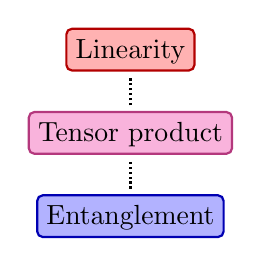
\begin{tikzpicture}[scale=0.6]
  \node[colorbox=red]                      (lin)  {Linearity};
  \node[colorbox=magenta, below=.5cm of lin] (tp)  {Tensor product};
  \node[colorbox=blue, below=.5cm of tp]   (en)  {Entanglement};
  \draw[conn=2pt, densely dotted] (tp) to (lin);
  \draw[conn=2pt, densely dotted] (en) to (tp);
\end{tikzpicture}
%			\caption{origin of entanglement via linearity}
%		\end{figure}
		
\section{Examples of key exchange}
	Exchanging keys for encryption was once done \textit{physically}, requiring the parties to meet and assure that no eavesdropper was present.
	Modern cryptographic systems make use of protocols over telecommunication channels. 
	In both cases the result at the end is that the trusted parties leave (or terminate the protocol) with a bit of information that they know it will be known only to them.\\
	Here we present examples for both classical and quantum mechanical channels and compare them.
		\subsection{The Diffie-Hellman key exchange}
		% Explain only how the protocol works, what is based on, what are its bounds, how it can be attacked (ideally).
		% Don't dive into Maurer violations, that will be covered in chapter [3] (XX)
	
		A famous and widely used method for the exchange of cryptographic keys is the Diffie-Hellman key-exchange method.
	The whole process can be summarized in five basic steps:
	\begin{enumerate}
		\item Alice and Bob \emph{publicly} communicate and agree on two numbers, that will serve as basis for the computations.
		\item Each party generates \emph{locally} a personal and distinct secret ($s_A$ and $s_B$) without ever communicating it .
		\item They mix their own secret with the common agreed basis, producing a result $R_A$ and $R_B$. The mathematical properties of this operation make it so it is computational infeasible to go back and retrieve the secrets $s$ from $R$.
		\item Both parties exchange \emph{publicly} their result. Each party now know both the result of the other and their own.
		\item Each party applies their secret to the received $R$. The outputs are equal for Alice and Bob so they can use this result as a common secret to create a key.
	\end{enumerate}	 
	
	The parts exchanged over the public channel --- the ones that Eve knows --- are only the mutually agreed base and the two partial mixtures. 
	It can be proven that those two elements alone give no information about the complete final shared secret and that it is virtually impossible to obtain the correct final product with only those two.\\  
	
	\subsection{The BB84 protocol}
	Protocols for the exchange of keys over a quantum channel have been invented.
	These protocols work on the underlying physics of quantum mechanics.
	Alice and Bob need then to have access to a quantum channel to exchange quantum states
	\footnote{A quantum channel is anything that can carry quantum states between two points. For example an optical fiber that carries photons.}.\\
	Here follows the BB84 protocol as described in \cite{NC10} :
		\begin{enumerate}
			\item Alice chooses $(4+\delta )n$ data bits.
			\item Alice chooses a random $(4+\delta )n$-bit string $b$. She encodes each data bit as $\{\ket{0},\ket{1}\}$ if the corresponding bit of $b$ is $0$ or with the diagonal basis if $b$ is $1$.
			\item Alice sends the resulting state to Bob.
			\item Bob receives the $(4+\delta )n$, announces \emph{publicly} this fact, and measures each qubit in the $X$ or $Z$ basis at random.
			\item Alice announces \emph{publicly} $b$.
			\item Alice and Bob discard any bits where Bob measured a different basis than Alice prepared. With high probability, there are at least $2n$ bits left (if not, abort the protocol and restart). They keep $2n$ bits.
			\item Alice selects a subset of $n$ bits that will to serve as a check on Eve's interference, and tells Bob which basis she selected.
			\item Alice and Bob announce \emph{publicly} and compare the values of the $n$ check bits. If more than an acceptable number disagree, they abort the protocol.
			\item Alice and Bob perform information reconciliation and privacy amplification on the remaining $n$ bits to obtain $m$ shared key bits.
		\end{enumerate}

	\subsection{The One-time Pad}
		%this is not really a method to share a common secret, since you have 
		% to already start with a secret.. <- point that out!
		
		% example of utilization of the key after generation
		% info theoretical key exchanged with OTP over already existing channel
		
		\begin{figure}[h!]
			\centering
			% OTP 
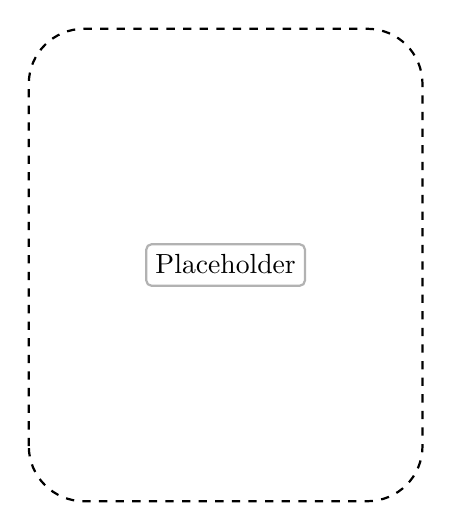
\begin{tikzpicture}
\draw[thick,dashed,rounded corners=.7cm] (-2.5,-3.) rectangle (2.5, 3);
\node[colorbox=white] (plc) at (0,0) {Placeholder};
\end{tikzpicture}



			\caption{Placeholder}
			\label{Fig:OTP}
		\end{figure}
\section{A comparison between securities}
    A point can be made comparing these different way of establishing privacy.
    The majority of cryptographic systems used are built on computational complexity security. 
    The so-called cryptographic functions are functions that are easy to compute in one way, but have a much higher complexity the other way round.\\
    
    This is the case for example for the Diffie-Hellman method. 
	The security in this method relies mainly on step 3.    
    Here an action as $ R_A = g^{s_A} \bmod p $ is performed, where $g$ and $p$ are the public common basis agreed beforehand. 
	To get back to $s_A$  one will need to find the prime factors of $R_A$, which is a known hard problem. 
	It is not impossible however. 
	The difficulty of breaking this step is bounded only by the length of the number chosen one one side and the computational power available to the adversary on the other.
	The access to the correlation between Alice and Bob is then shielded against Eve only by the assumption that she does not have enough computational power to break it.\\
	
	The BB84 works differently. 
	It takes advantage of the monogamy of entanglement. 
	If Eve was able to wire-tap the quantum channel, she would disrupt the correlation between Alice and Bob.
	Despite this protocol seems impossible to break, ...
	
    
\section{The equivalent of CKA in QM}
	What we were trying to do was to factor out Eve from Alice and Bob's point of view.
	The goal of classical key agreement (CKA) is also to create a private correlation between Alice and Bob, from one that also includes Eve.\\
	We already stated that entangled states can provide this level of privacy.
	However pure entangled states are very fragile and do not occur in nature.
	The more general quantum state is a mixed state.
	A mixed state is a composition of pure states with their probability.
	\begin{equation}
		\rho = \sum_i p_i \ketbra{\psi_i}{\psi_i} ,\quad \ket{\psi_i}: \text{ state with probability } p_i
	\end{equation}
	Assume that Alice and Bob start with a state $\rho$ which is also mixed with a part owned by Eve. 
	Is there a way to factor her out the state?
	Quantum distillation is a process that allows that. 
%	Through a series of local operations and classic (public) communication, Alice and Bob can indeed reach a new state $\rho_{AB}$ that has the state $\rho_E$ of Eve factored out.
	Maximally entangled states held between Alice and Bob after a distillation protocol are --- by the monogamy of entanglement --- not entangled with the environment. 
	In other words, the state Alice and Bob have is product with the environment.\\
	The joint probability distribution $P_{ABE}$ falls similarly into a product $P_{AB}\cdot P_E$ after a CKA protocol.\\
    
    \begin{figure}[h]
    	\centering
    	% Image showing intuition process
% Sort of justify how and why 
% bound entanglement and bound information
% should share analogies

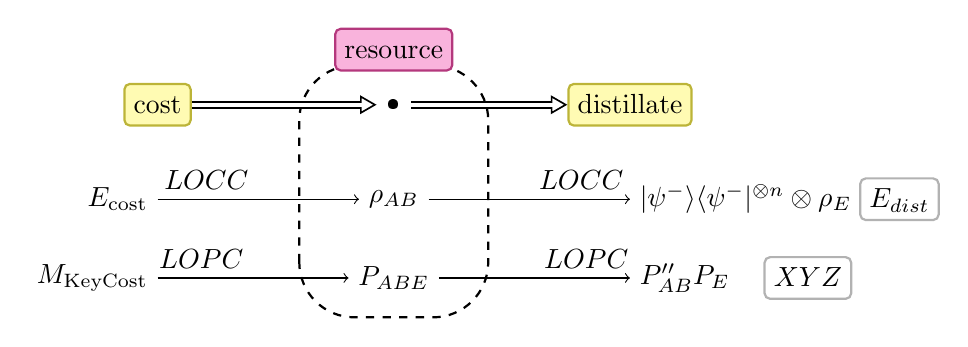
\begin{tikzpicture}
\tikzstyle{vecArrow} = [thick, decoration={markings,mark=at position
   1 with {\arrow[semithick]{open triangle 60}}},
   double distance=1.4pt, shorten >= 5.5pt,
   preaction = {decorate},
   postaction = {draw,line width=1.4pt, white,shorten >= 4.5pt}]
\tikzstyle{fancyArrow} = [<->,very thick,decorate,decoration={snake,amplitude=.4mm,segment length=2mm,post length=1mm}]

	\coordinate (center) at (0,0);
	\draw[thick,dashed,rounded corners=.7cm] (-1.20,-1.) rectangle (1.20, 2.2);
	\node[colorbox=yellow] (cst) at (-3,1.7) {\strut cost};
	\node[colorbox=yellow, baseline=(cst.baseline)] (dst) at (3,1.7) {\strut distillate};
	\node[colorbox=magenta, baseline=(cst.baseline)] (rsc) at (0.0, 2.4) {\strut resource};
	\node[anchor=center, left] (ecost) at (-3,0.5) {$E_{\text{cost}}$};
	\node[anchor=center] (rho) at (0.0,0.5) {$\rho_{AB}$};
	\node[anchor=center, right] (distilled) at (3,0.5) {$\ketbra{\psi^{-}}{\psi^{-}}^{\otimes n}\otimes \rho_E$};
	\node[colorbox=white, right=of distilled, anchor=east] (edist) {$E_{dist}$};
	
	\node[anchor=center, left] (kcost) at (-3,-0.5) {$M_{\text{KeyCost}}$};
	\node[anchor=center] (prob) at (0.0,-0.5) {$P_{ABE}$};
	\node[anchor=center, right] (ckey) at (3,-0.5) {$P''_{AB}P_E$};
	\node[colorbox=white, right=of ckey.center] (skr) {$\keyrate{X}{Y}{Z}$};
	
	\node[thick, baseline=(cst.baseline)] (bul) at (0.0, 1.7) {\strut\textbullet};
%	\node[above=of bul] (res) {Resource (fixed)}; 
	

	\draw[vecArrow] (cst.east) to (bul.west);
	\draw[vecArrow] (bul.east) to (dst.west);
	\draw[->] (ecost) to node[above left]{$LOCC$} (rho); \draw[->] (rho) to node[above right]{$LOCC$} (distilled);
	\draw[->] (kcost) to node[above left]{$LOPC$} (prob); \draw[->] (prob) to node[above right]{$LOPC$} (ckey);

\end{tikzpicture}

    	\caption{Entanglement distillation and CKA utilise a resource (mixed state or probability distribution) to produce a distillate that factors out Eve.}
    	\label{Fig:intuition}
    \end{figure}
    
    To measure entanglement one might consider the least number of maximally entangled bipartite quantum states required to prepare a density matrix $\rho$ by local operations and classical communication. 
    Similarly one might measure entanglement by the maximal number of singlets that can be obtained form $\rho$ by local operations and classical communication. 
    These measures are not the same. 
    The first is called \emph{entanglement cost} or entanglement of formation; the second describes the distilled state. 
    The classical counterpart would be the \emph{information of formation} and the \emph{secret-key rate}.\\
    Figure \ref{Fig:intuition} illustrates the analogy between the resource, distillate and cost.
    This is part of the intuition that leads to bound information.
    
    
		
\chapter{Bound Information}
\section{Conjectures}
% Here you can retake the examples of protocols in chapter 1. After explaining Maurer postulate, show that they don't violate Maurer because of reasons.
			\begin{quotation}
			Bound entanglement is a kind of correlation between Alice and Bob inaccessible to Eve but nevertheless of no use for generating a secret (quantum) key.\\
			Unfortunately the existence of such bound information, which would contradict the mentioned conjecture\footnotemark on the classical side of the picture, could not be proven so far.
		\end{quotation}
		
		\footnotetext{Shannon: Information theoretical security can be achieved only by parties sharing an unconditionally secret key initially. Maurer: this key can also not be generated from scratch. Maurer+Wolf: \emph{Intrinsic information} between $A$ and $B$ given $E$ == \emph{secret key rate}(how much key can Alice and Bob generate from that $P_{ABE}$).}
		
	%\lipsum[1]
	\section{State of research}
		\begin{figure}[h]
			\centering
			% scheme representing the bounds
% expresed in paper Renner+Wolf 2003
% on the quantities intrinsic information,
% secret key rate and information of formaion

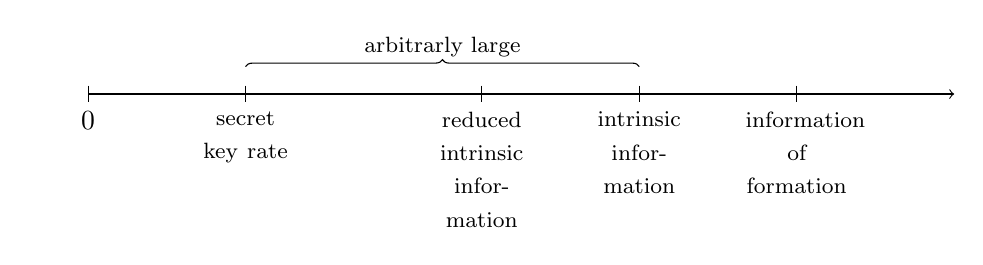
\begin{tikzpicture}
%	\tikzstyle{lineLabel}=[text width=10mm,align=center, below]
%	\draw[->] (0,0) -- (11,0);
%	\draw (0,.5) -- (0,-.5);
%	\draw (2,.5) -- (2,-.5);
%	\draw[dashed] (5,.5) -- (5,-.5);
%	\draw (7,.5) -- (7,-.5);
%	\draw (9,.5) -- (9,-.5);
%	
%	\node (zero) at (0,-.7) {$0$};
%	\node[lineLabel] (iof) at (9,-.7) {\footnotesize Information of formation};
%	\node[lineLabel] (inf) at (7,-.7) {\footnotesize Intrinsic Information};
%	\node[lineLabel] (rinf) at (5,-.7) {\footnotesize Reduced Intrinsic Information};
%	\node[lineLabel] (skr) at (2,-.7) {\footnotesize secret key rate};

\tikzset{
    position label/.style={
       below = 3pt,
       align=center,
%       text height = 1.5ex,
%       text depth = 1ex,
       text width=13mm
    },
   brace/.style={
     decoration={brace},
     decoration={raise=3ex},
     decorate
   },
   blabel/.style={
		above = 13pt,
		align=center,
		pos=0.5   
   }
}

% draw horizontal line
\draw[->] (0,0) -- (11,0);

%draw vertical lines
\foreach \x in {0,2,5,7,9}
   \draw (\x cm,3pt) -- (\x cm,-3pt);

%labels
\node [position label] (Start) at (0,0) {$0$};
\node [position label] (skr) at (2,0) {\footnotesize secret key rate};
\node [position label] (rinf) at (5,0) {\footnotesize reduced intrinsic information};
\node [position label] (inf) at (7,0) {\footnotesize intrinsic information};
\node [position label] (iof) at (9,0) {\footnotesize information of formation};

\draw [brace] (skr.north) -- node [blabel] {\footnotesize arbitrarly large} (inf.north);

\end{tikzpicture}
			\caption{Bounds on the quantities as stated in Wolf + Renner 2003 proceeding}
		\end{figure}
	%\lipsum[1]
	\section{My considerations}
	%\lipsum[1]

	
%\chapter{Conclusion}
%%

%\bibliographystyle{apalike}
\printbibliography
\end{document}
